\documentclass{beamer}
\usepackage{default}
\usepackage{pgfpages}
\usepackage{tikz}
\usepackage{mathtools}
\renewcommand{\thefootnote}{}
\usepackage{colortbl}
\usepackage{hyperref}
\usepackage{multimedia}
\title{Git Review}
\begin{document}


\begin{frame}
\begin{center}
Introduction to Version Control with \texttt{Git}
\end{center}
\end{frame}

\begin{frame}
\frametitle{Why do I need version control?}
\end{frame}


\begin{frame}
\frametitle{Why do I need version control?}
\begin{center}
\scalebox{0.4}{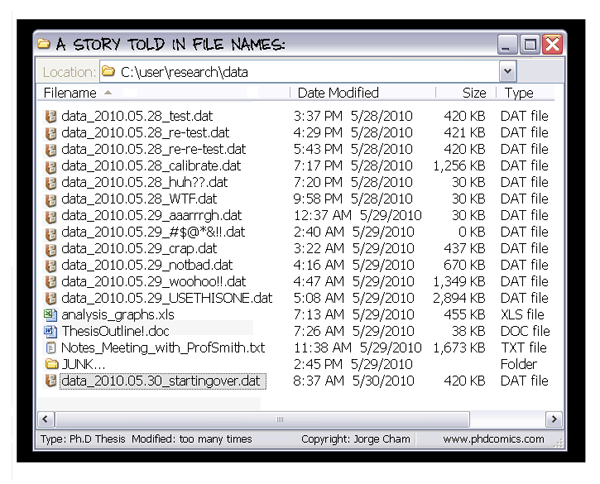
\includegraphics{../imgs/version_control.png}}
\end{center}
\footnote{\footnotesize{https://www.phdcomics.com}}
\end{frame}

\begin{frame}
\frametitle{Why do I need version control?}
\begin{itemize}
\item Make changes to code with confidence - \textit{can always be reverted if necessary} \pause
\item Reproducibility -  \textit{version control can complement your lab notebook} \pause
\item Work as a team -  \textit{file names and directory structures are consistent for all team members} \pause
\item The list goes on...
\end{itemize}
\end{frame}

%\begin{frame}
%\frametitle{Goals for today:}
%\begin{itemize}
%\item Learn the \textit{workflow} and \textit{\textbf{vocabulary}} of version control with  \texttt{Git} \pause
%\begin{itemize}
%\item Disclaimer: this is hard \pause
%\end{itemize}
%\item Learn how to collaborate with Github \pause
%\begin{itemize}
%\item Disclaimer: this is also hard \pause
%\end{itemize}
%\item Ultimately enable you to figure out what you want to do with \texttt{Git} 
%\end{itemize}
%\end{frame}

\begin{frame}
\frametitle{\texttt{Git}}
In the scientific world, Git (and Github) is the most widely used version control system.
\begin{center}
\scalebox{0.4}{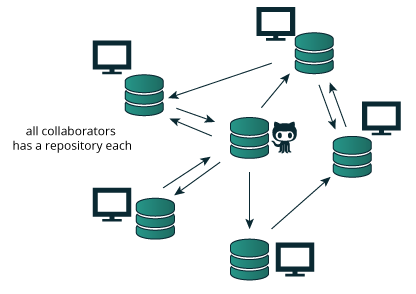
\includegraphics{../imgs/distributed-vc.png}}
\end{center}\pause
\textit{\textcolor{red}{repository}:} A central storage area where a version control system stores old revisions of files and information about who changed what, when.
\footnote{\footnotesize{http://invistruct.com/}}
\end{frame}

\begin{frame}[fragile]
\frametitle{How do you get your own repository?}
Let's configure \texttt{Git} first:
\begin{verbatim}
$ git config --global user.name "Your name goes here"
$ git config --global user.email you@yourdomain.com
$ git config --global core.editor vim
$ git config color.ui auto
\end{verbatim}
Then initialize your first repository:
\begin{verbatim}
$ git init
\end{verbatim}
\begin{center} \pause
\textbf{You Try (10 minutes):}

\textbf{\textcolor{red}{Exercises (1) - 2}}
\end{center}
\end{frame}


\begin{frame}
\frametitle{\texttt{Git} allows you to save snapshots of your directory}
% One of the main goals of version control is to save snapshots of your directory
\textit{\textcolor{red}{commit}}: snapshots of your directory. \pause
\begin{itemize}
\item There is metadata associated with each commit (snapshot): 
\begin{itemize}
\item the date the snapshot was taken
\item who took it
\item what files were modified
\item the changes made on those files
\item etc. 
\end{itemize}\pause
\item \texttt{Git} will enable you to:
\begin{itemize}
\item track the changes made to files in your directory
\item revert the entire project to a previous snapshot
\item review changes made over time
\item view who modified a file
\item etc. 
\end{itemize}
\end{itemize}
\end{frame}

\begin{frame}
\frametitle{A little more vocabulary:}
There are three main \textit{trees} or \textit{collections of files (and metadata)} in \texttt{Git}:
\begin{center}
\scalebox{0.4}{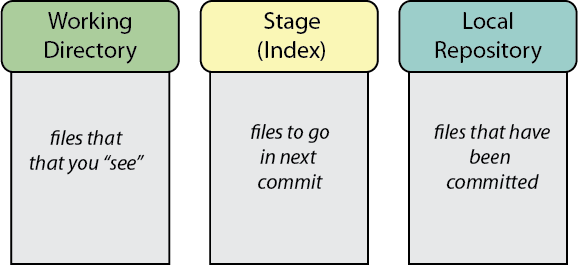
\includegraphics{../imgs/three_trees_of_git.png}}
\end{center}
\end{frame}

\begin{frame}
\frametitle{How to save snapshots with \texttt{Git}}
\begin{center}
\scalebox{0.4}{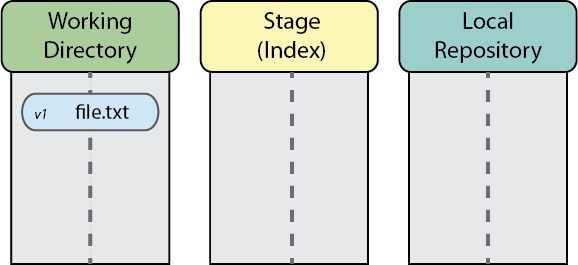
\includegraphics{../imgs/work.png}}
\end{center}
\end{frame}

\begin{frame}
\frametitle{How to save snapshots with \texttt{Git}}
\begin{center}
\scalebox{0.4}{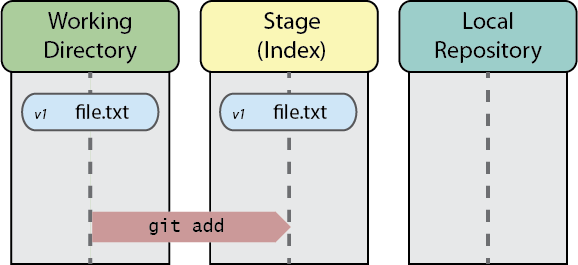
\includegraphics{../imgs/work_add.png}}
\end{center}
\end{frame}

\begin{frame}
\frametitle{How to save snapshots with \texttt{Git}}
\begin{center}
\scalebox{0.4}{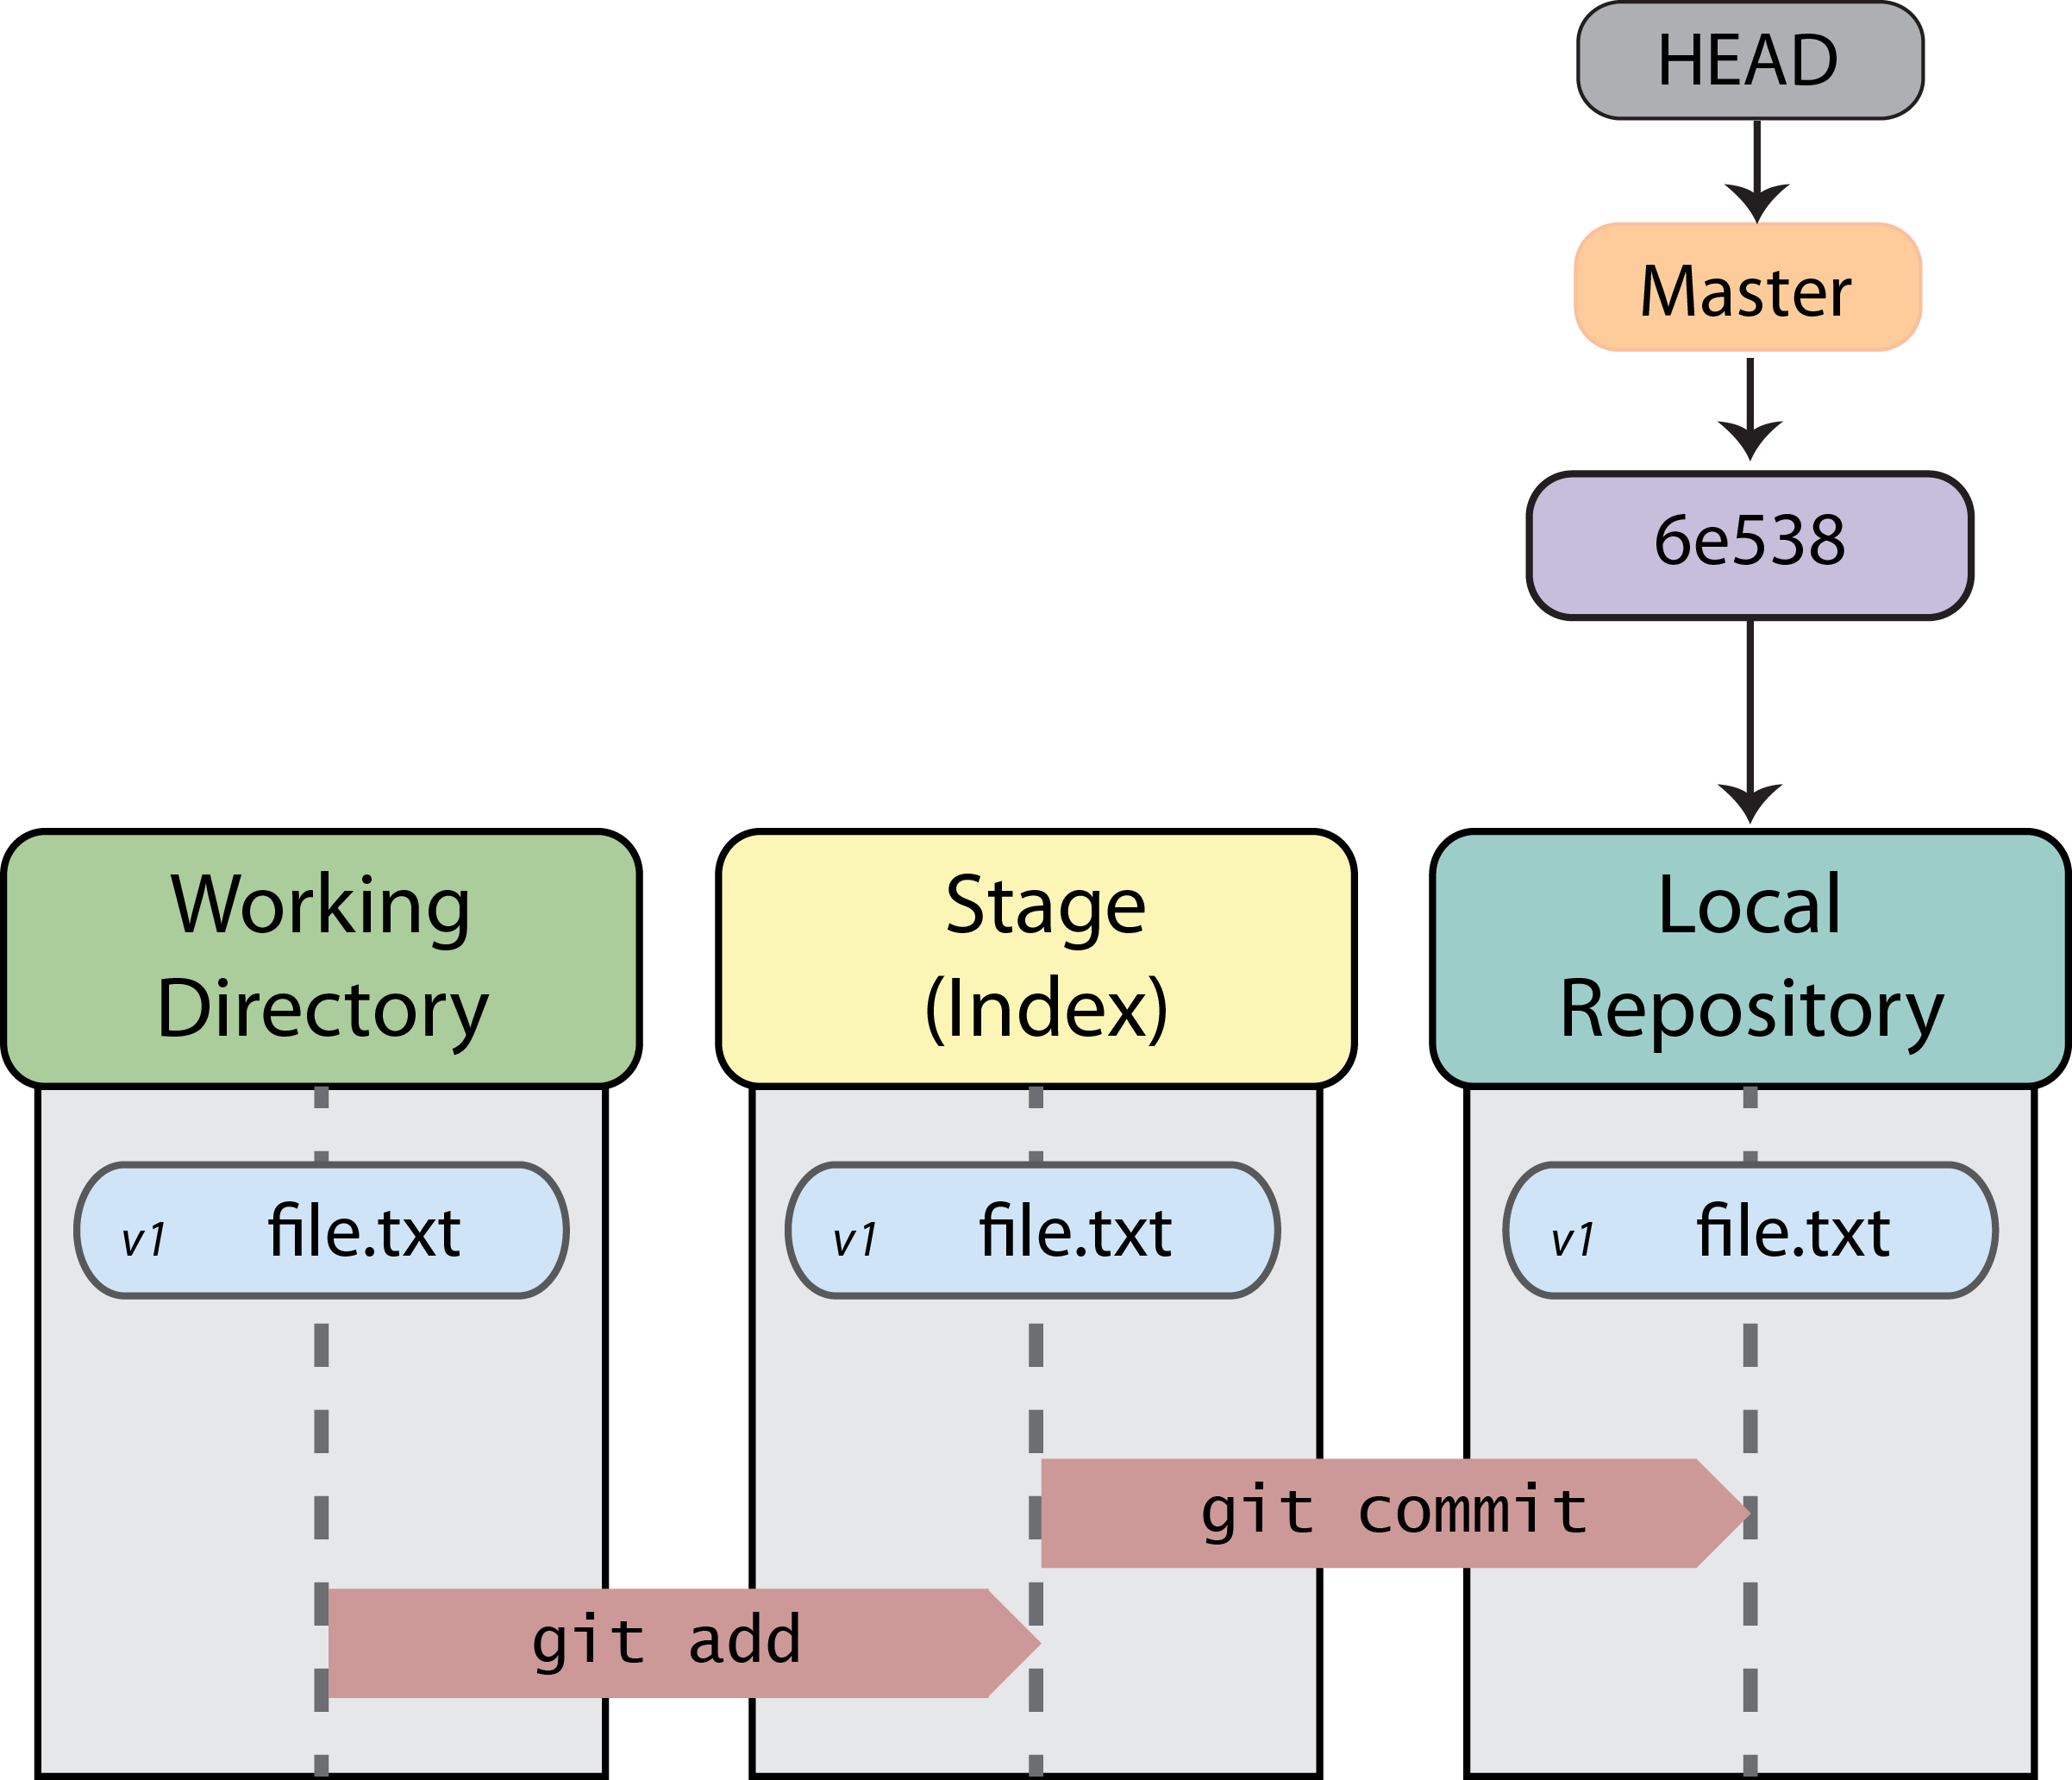
\includegraphics{../imgs/work_add_commit.png}}
\end{center}
\end{frame}

\begin{frame}
\frametitle{How to save snapshots with \texttt{Git}}
\textit{\textcolor{red}{SHA-1 hash:}} \textit{unique} 40-digit computer-generated identifier for each revision (or commit)
\begin{center}
\scalebox{0.3}{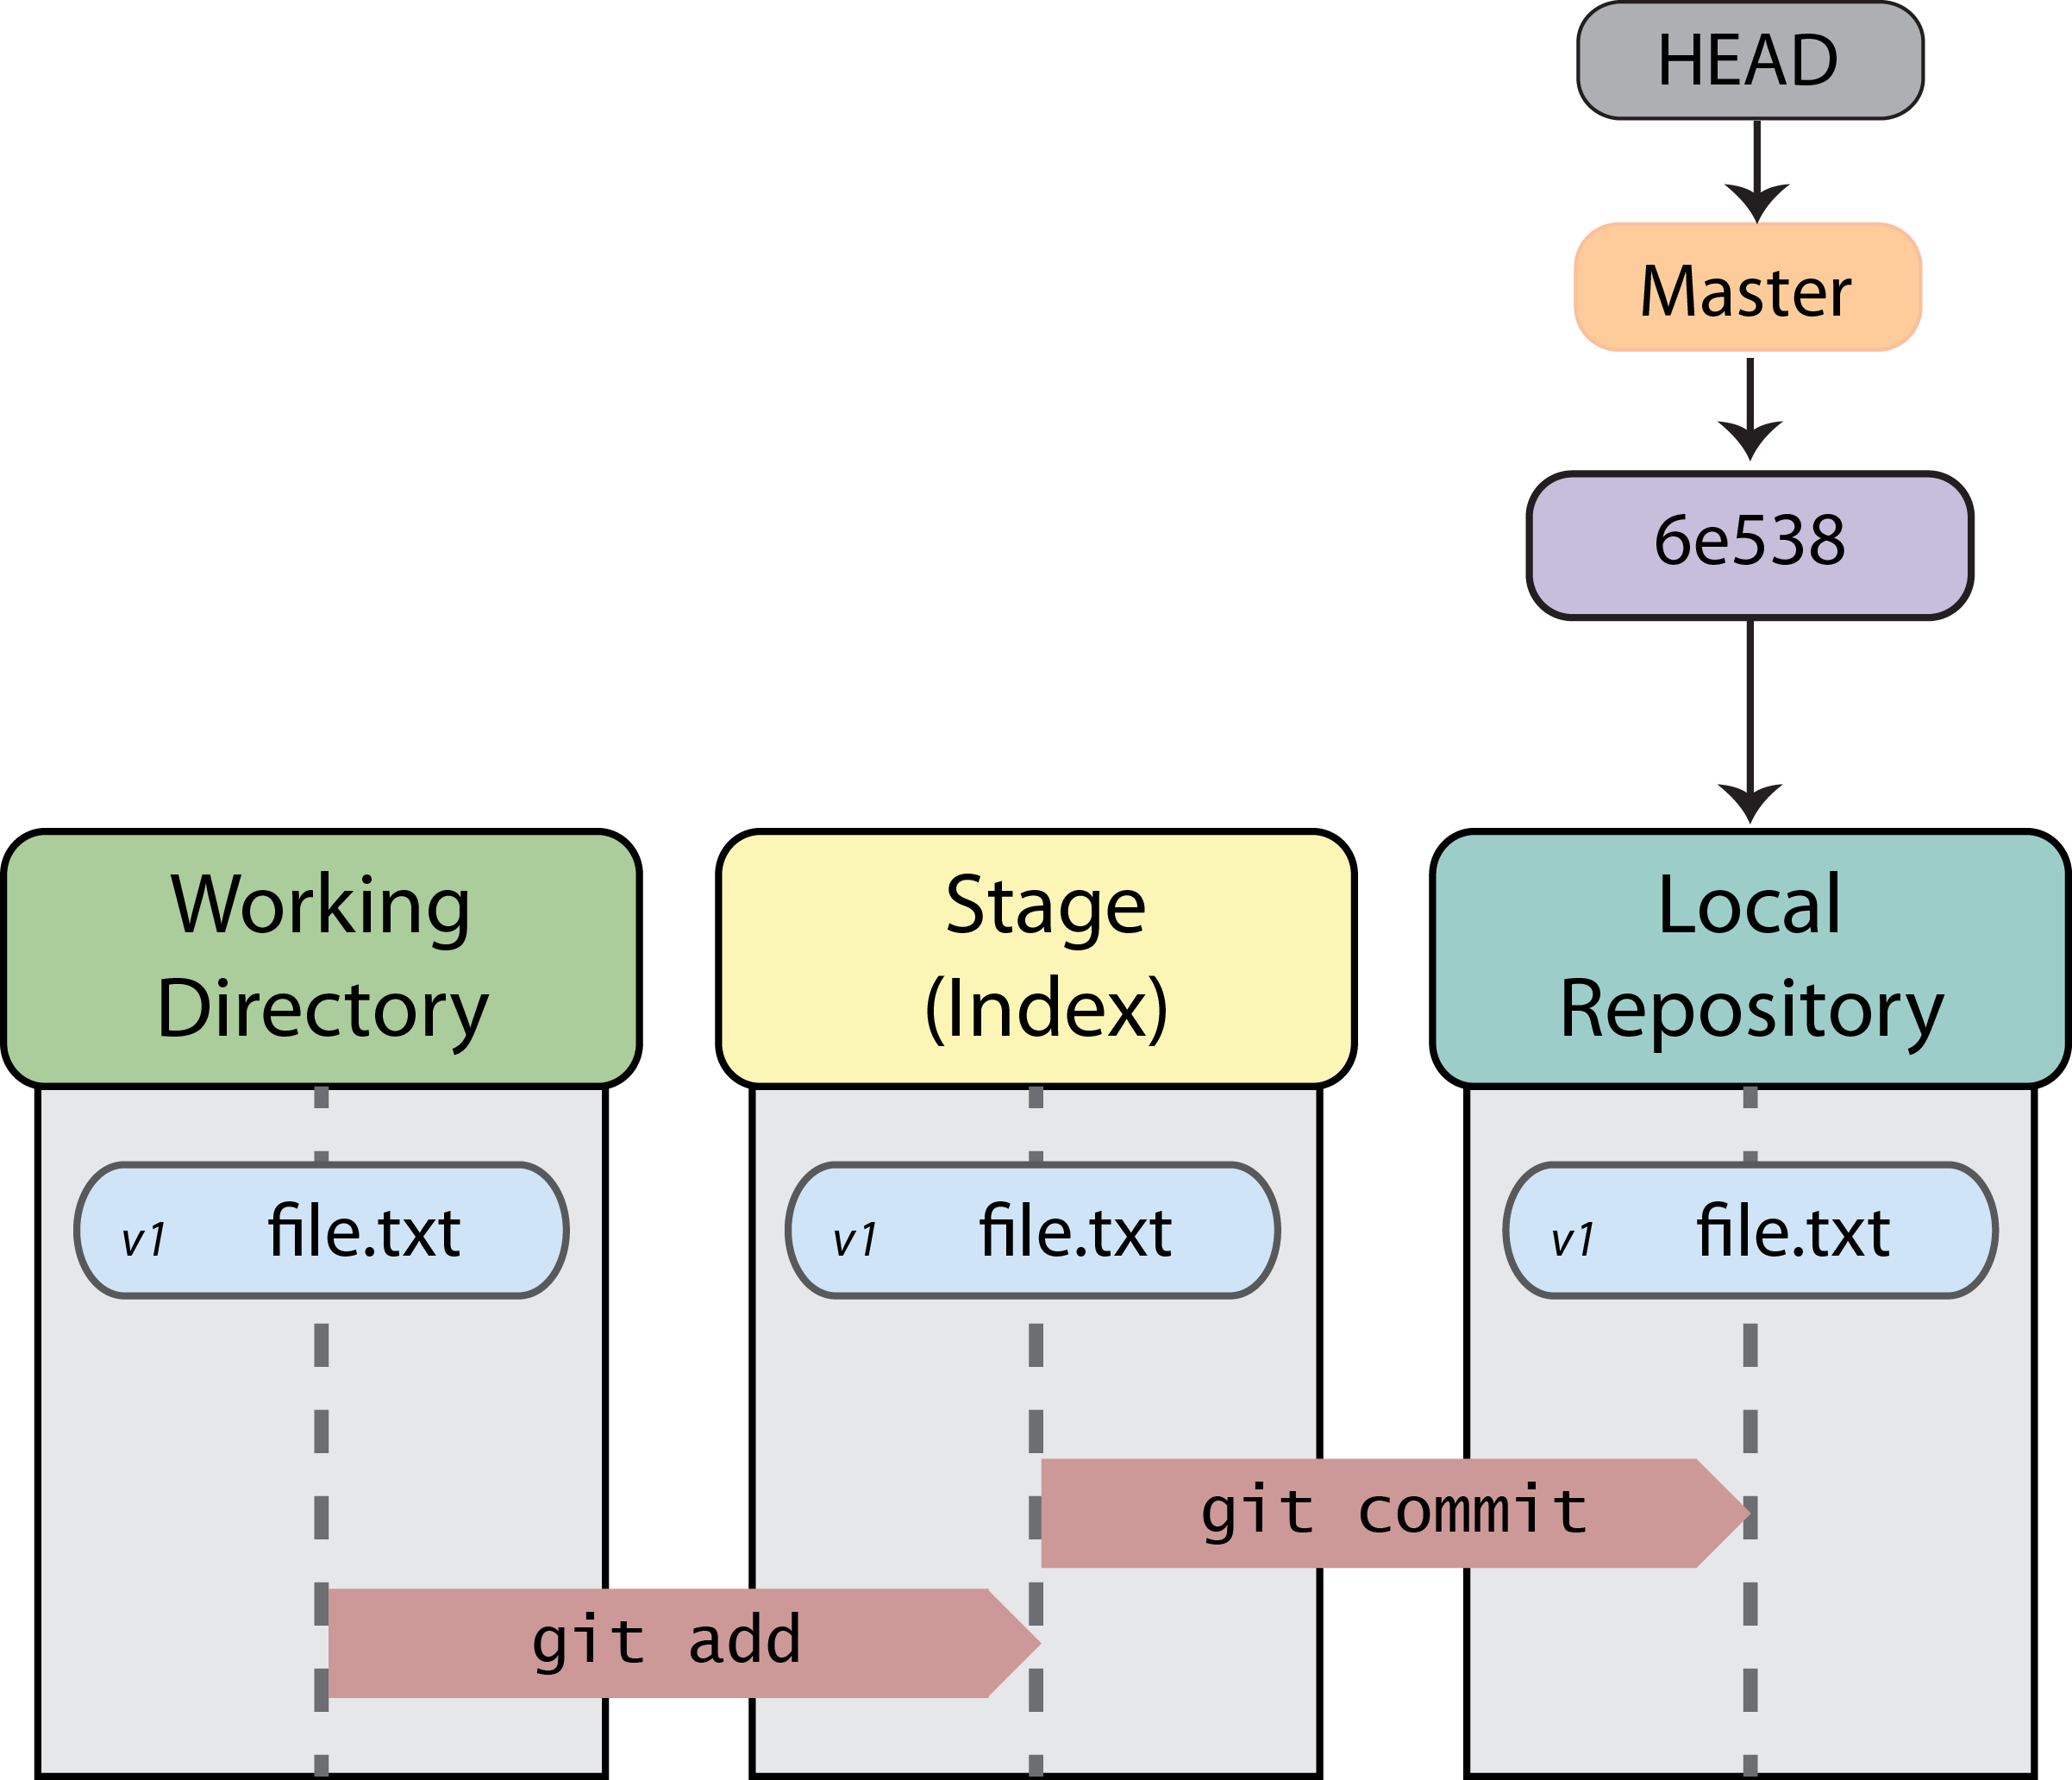
\includegraphics{../imgs/work_add_commit.png}}
\end{center}
\end{frame}

\begin{frame}
\frametitle{How to save snapshots with \texttt{Git}}
\textit{\textcolor{red}{SHA-1 hash:}} \textit{unique} 40-digit computer-generated identifier for each revision (or commit)

\textit{\textcolor{red}{HEAD:}} reference to the current branch or commit
\begin{center}
\scalebox{0.3}{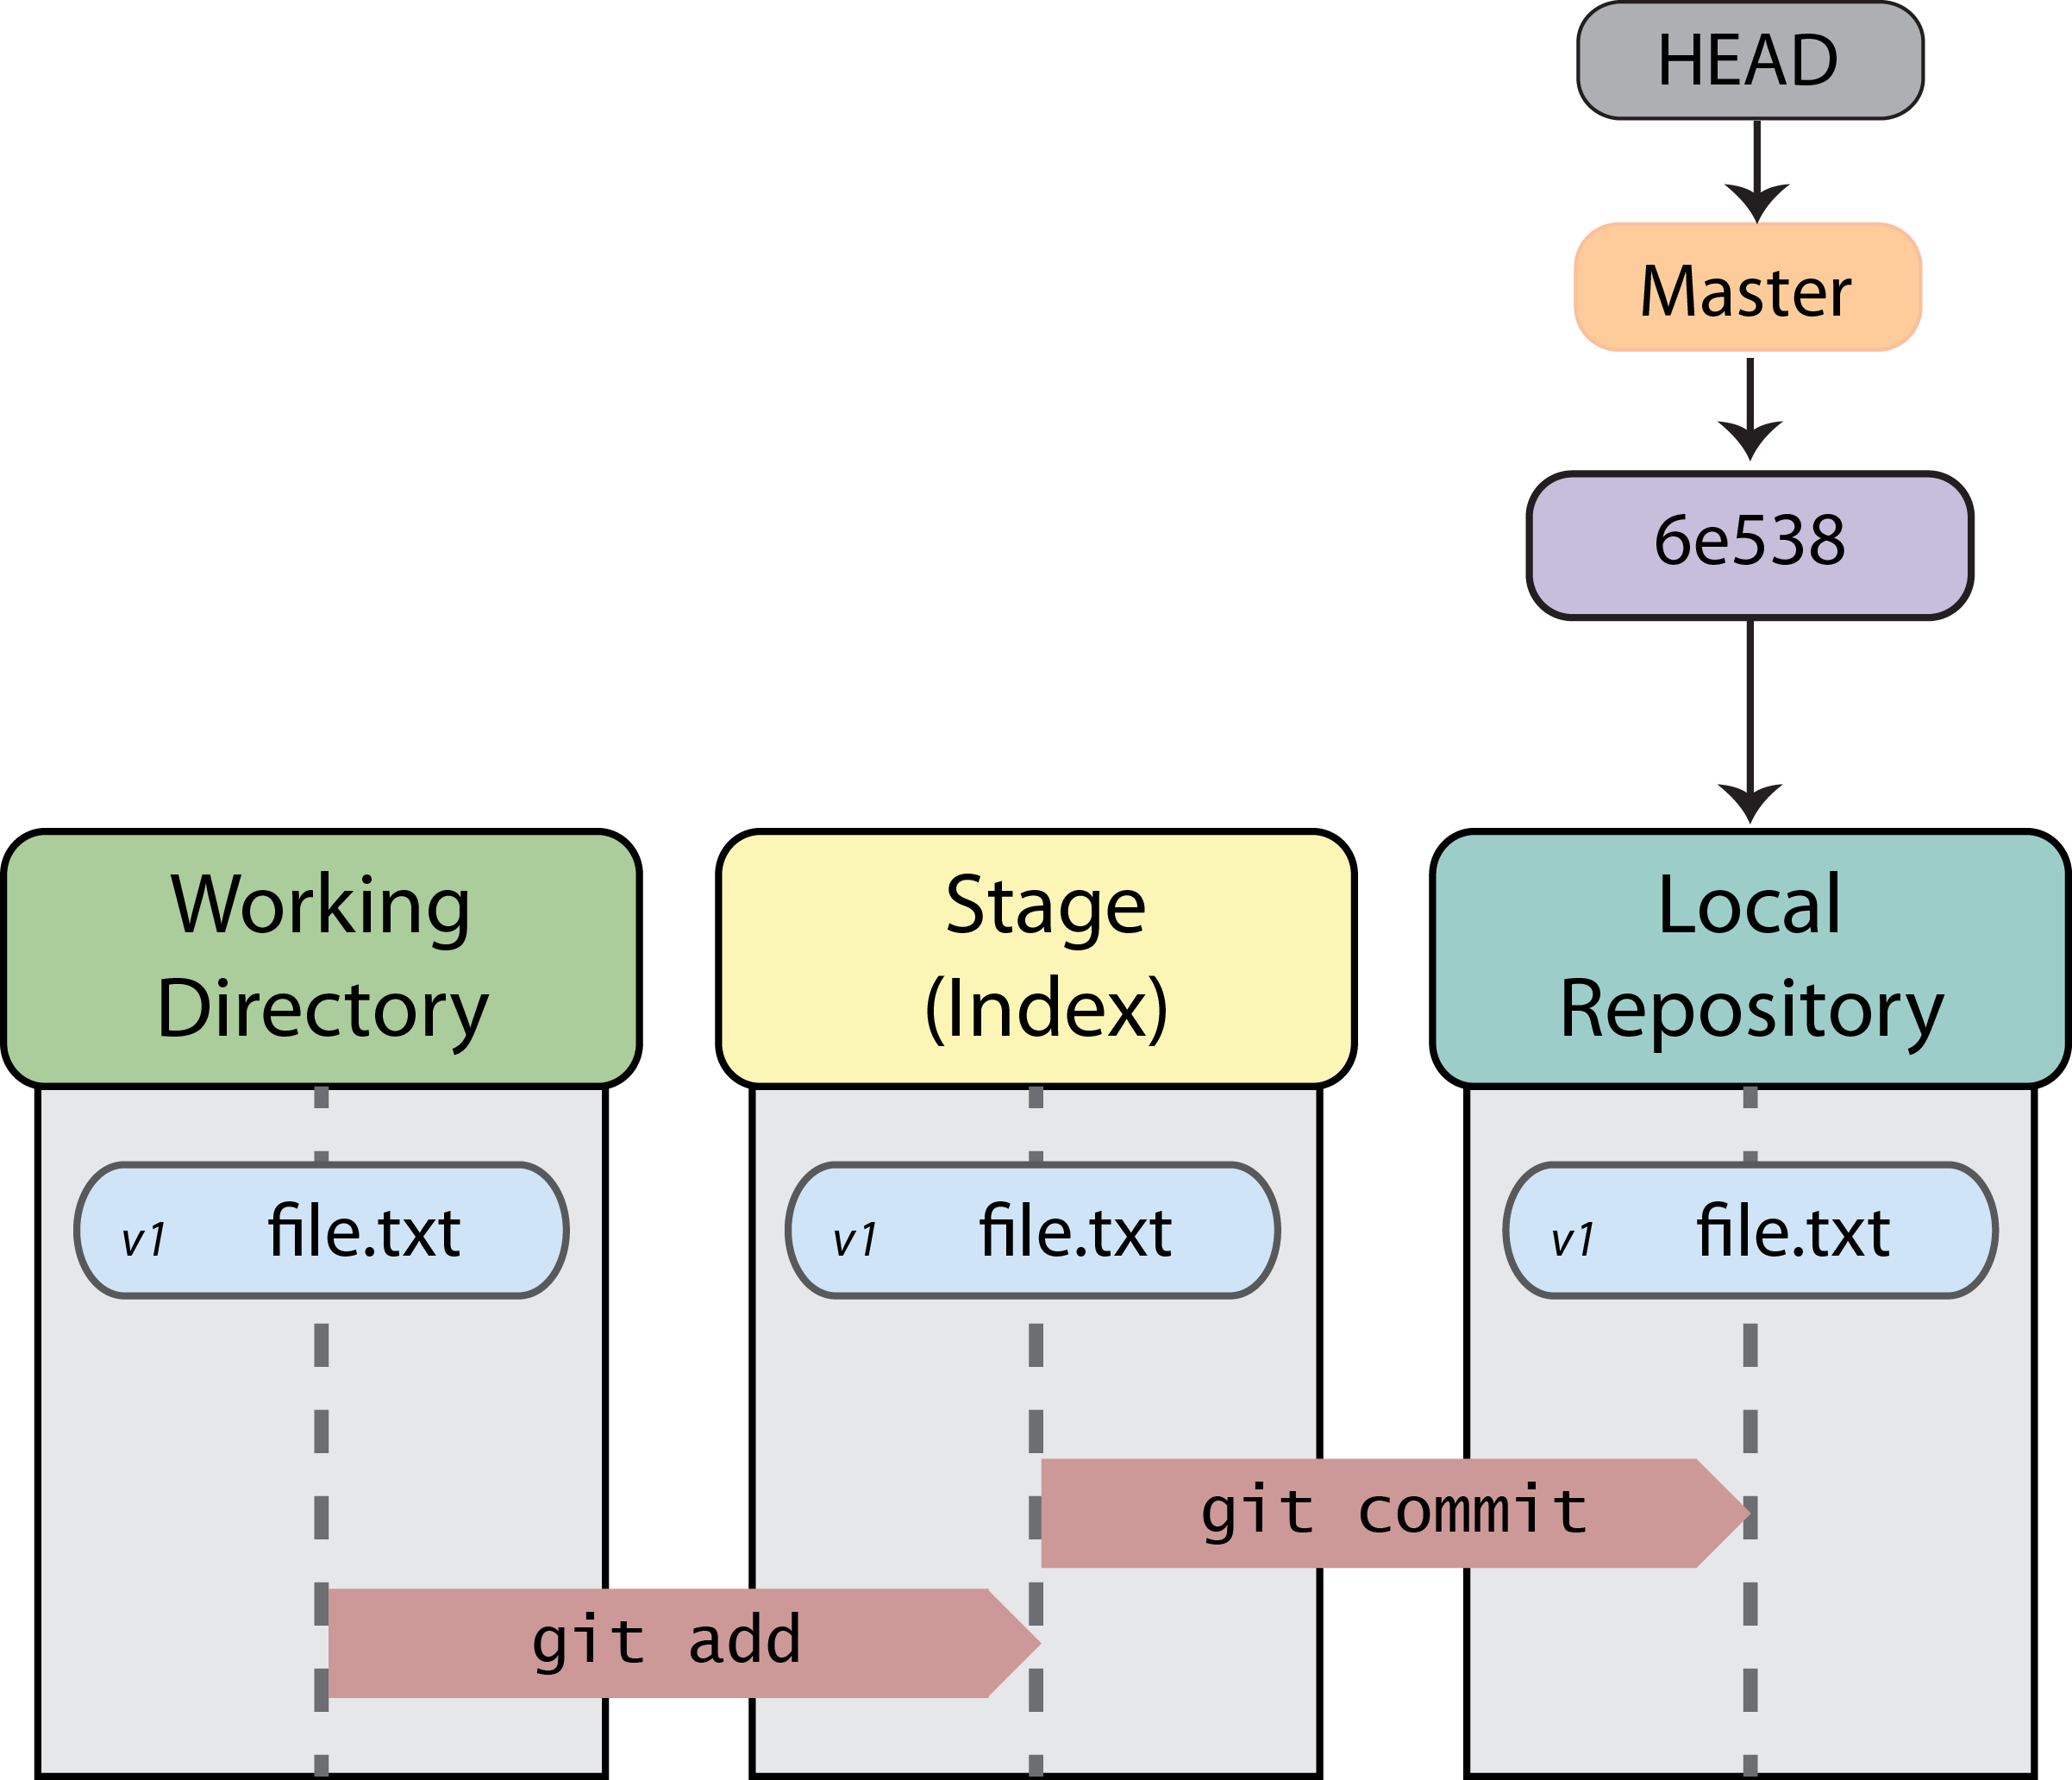
\includegraphics{../imgs/work_add_commit.png}}
\end{center}
\end{frame}

\begin{frame}
\frametitle{How to save snapshots with \texttt{Git}: Keep working!}
\begin{center}
\scalebox{0.4}{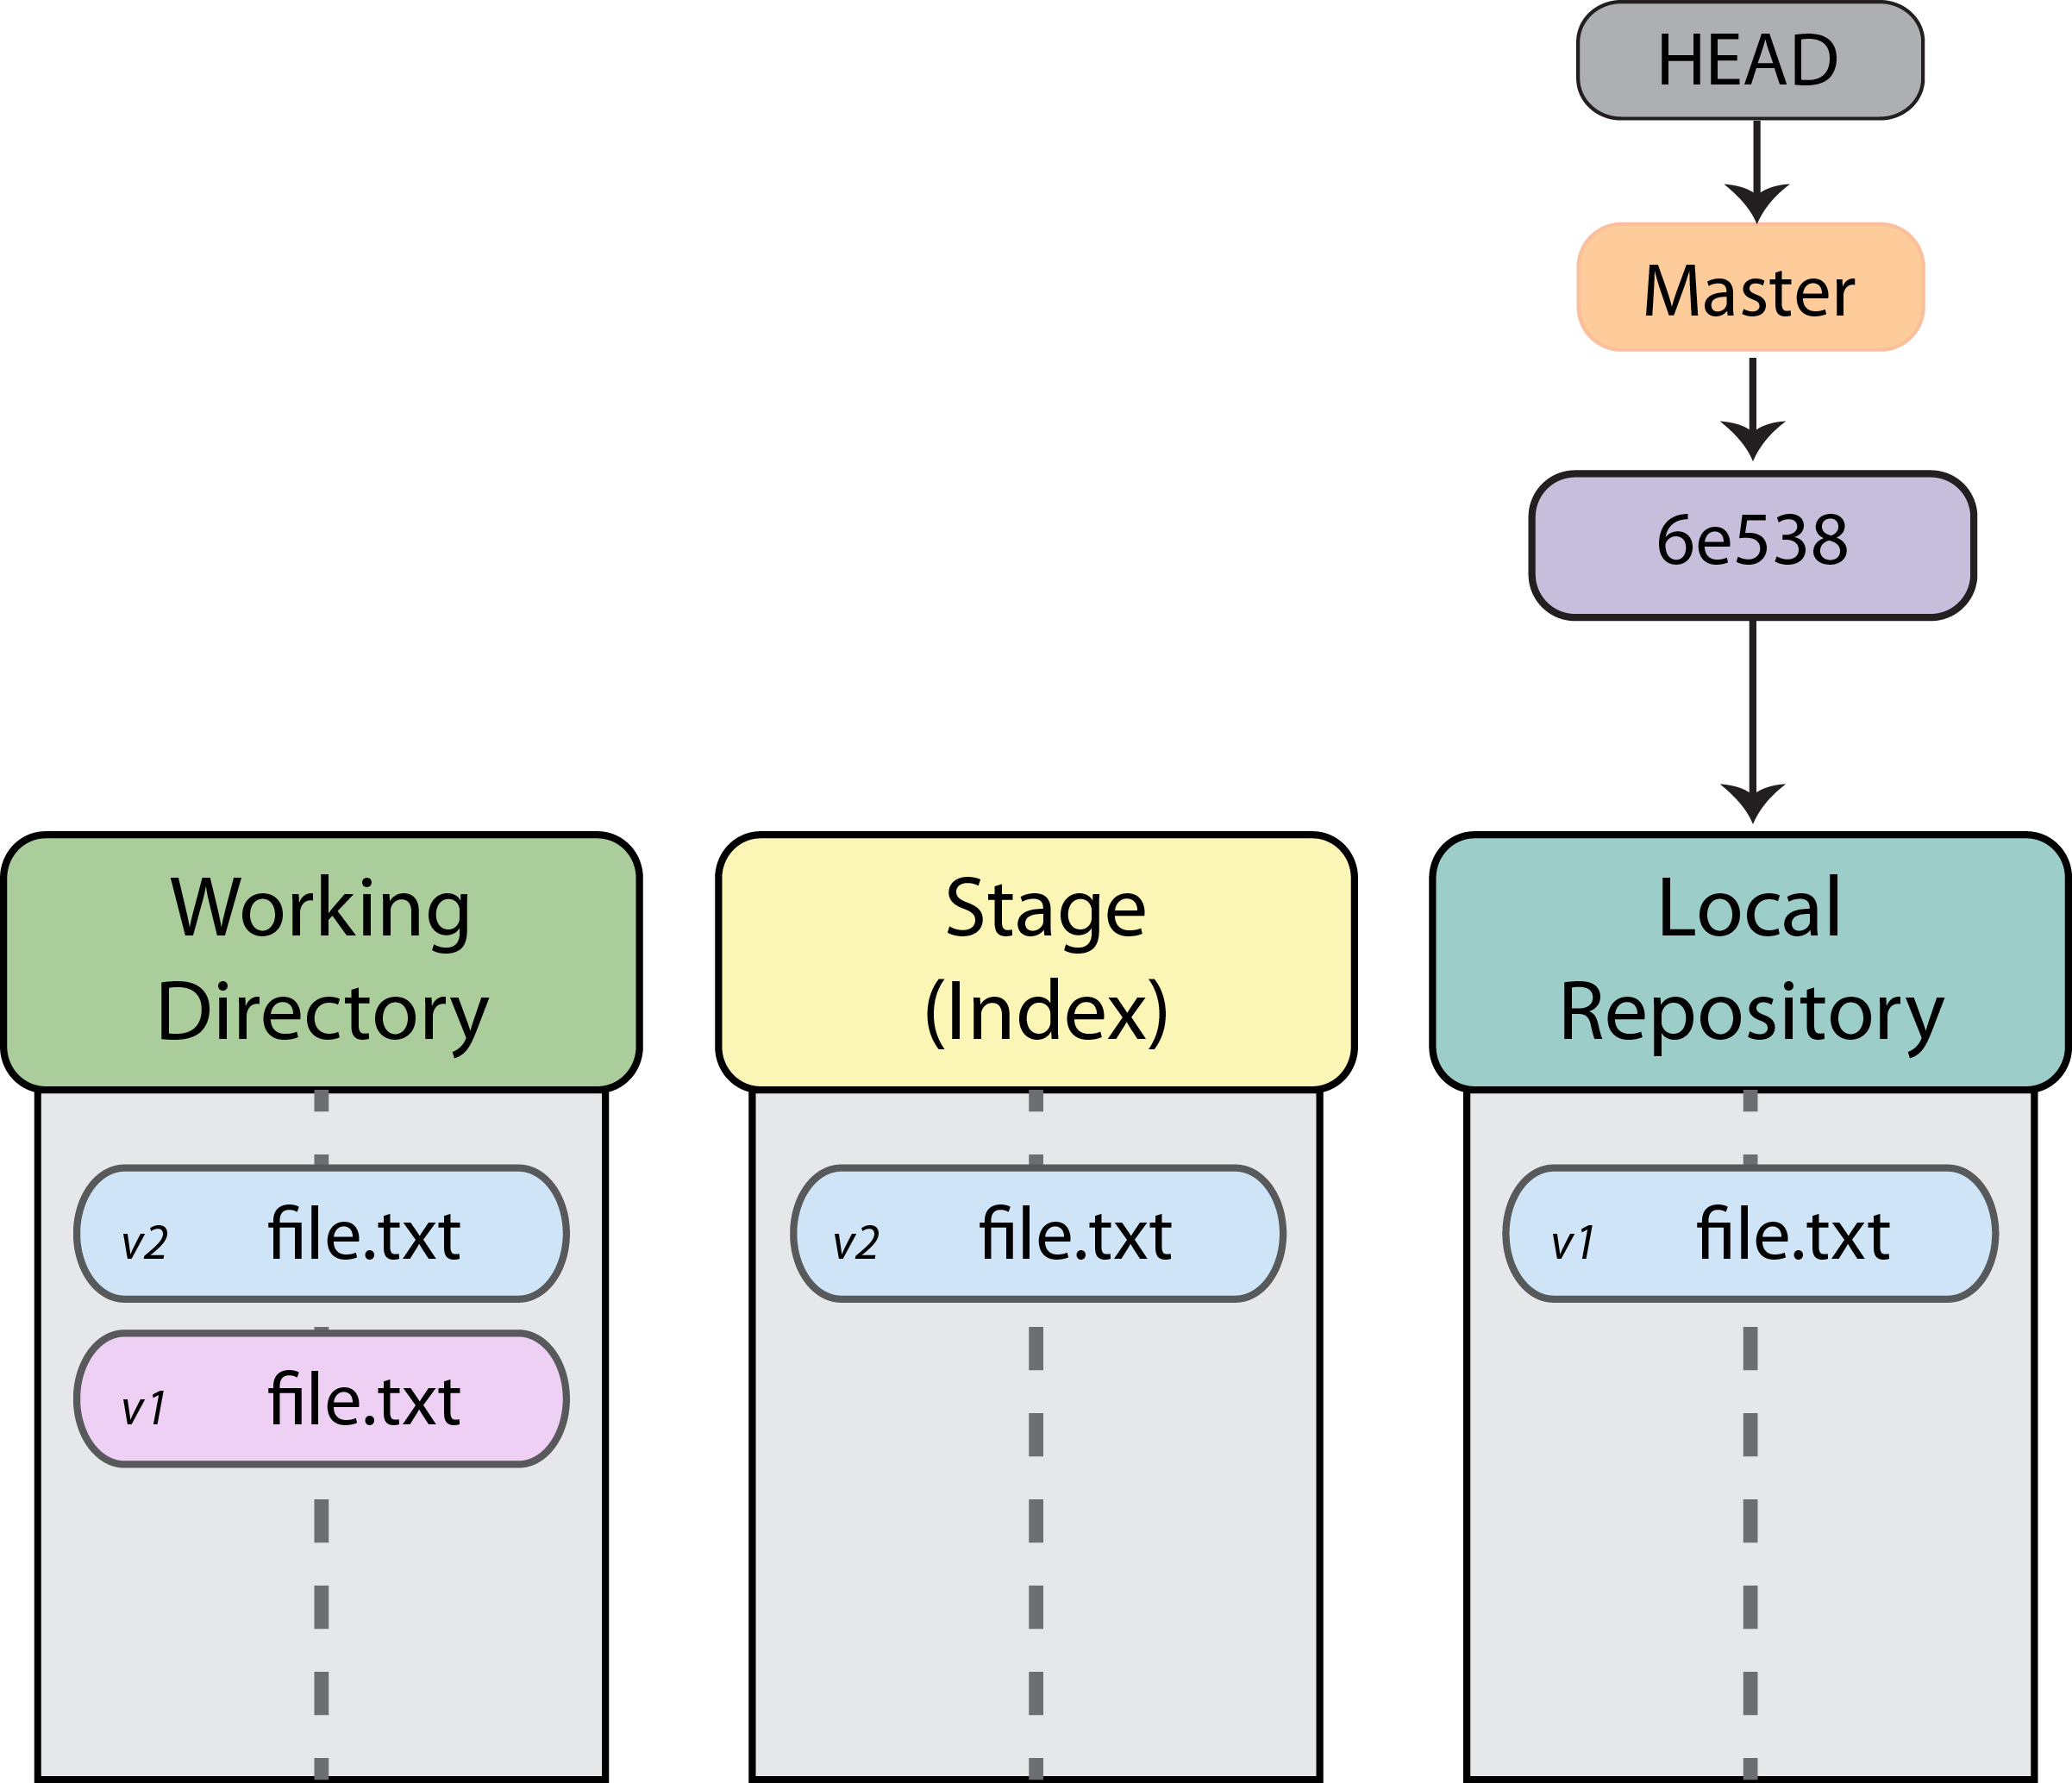
\includegraphics{../imgs/work_add_commit_work.png}}
\end{center}
\end{frame}

\begin{frame}
\frametitle{How to save snapshots with \texttt{Git}: Keep working!}
\begin{center}
\scalebox{0.4}{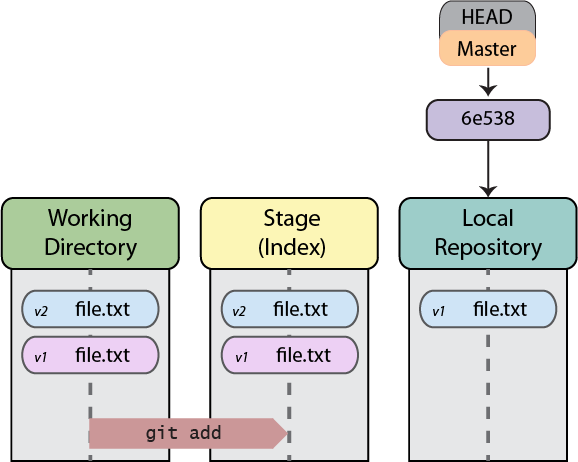
\includegraphics{../imgs/work_add_commit_work_add.png}}
\end{center}
\end{frame}

\begin{frame}
\frametitle{How to save snapshots with \texttt{Git}: Keep working!}
\begin{center}
\scalebox{0.4}{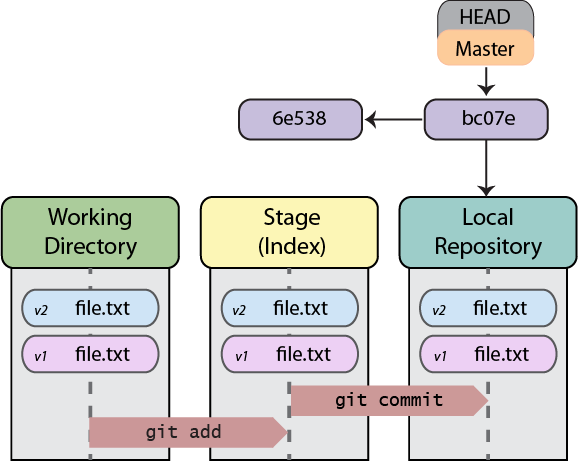
\includegraphics{../imgs/work_add_commit_work_add_commit.png}}
\end{center}
\end{frame}


\begin{frame}
\frametitle{A simple story so far: what else can we do?!}
\texttt{git log}: view the change history (commits) of the current repository.

\end{frame}

\begin{frame}
\frametitle{A simple story so far: what else can we do?!}
\texttt{git diff}: view changes between files and commits
\begin{center}
\scalebox{0.4}{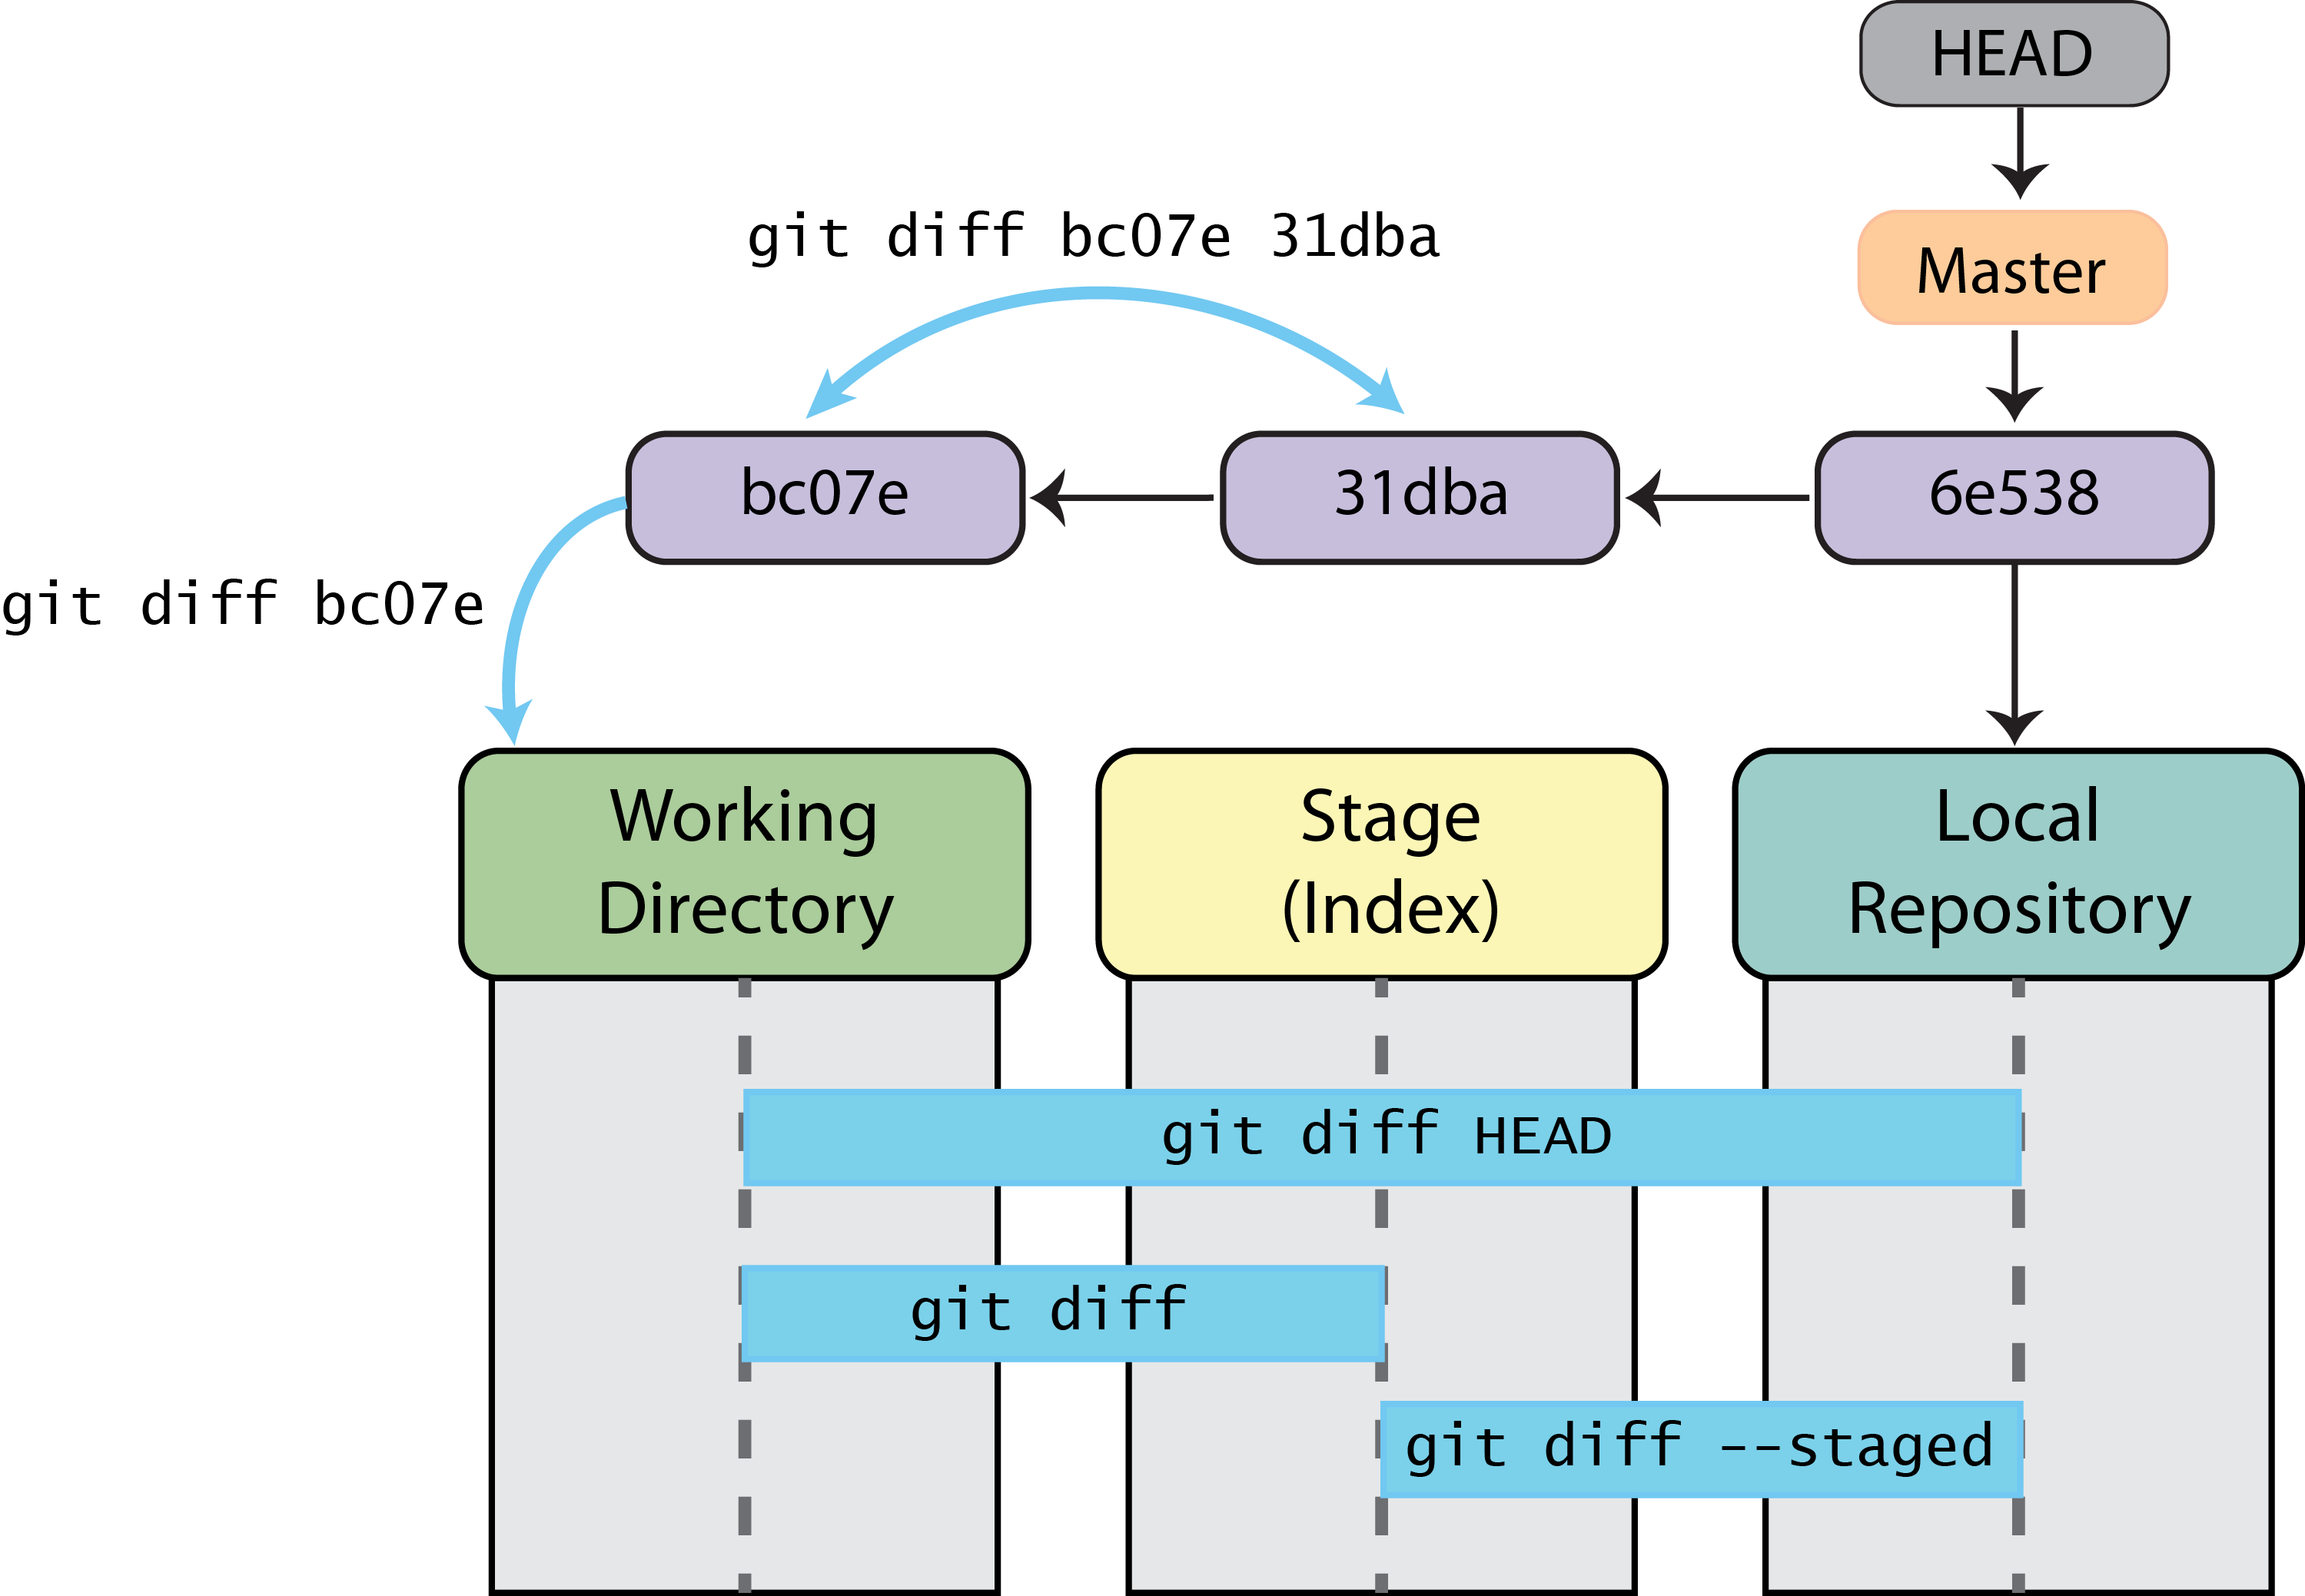
\includegraphics{../imgs/diff_commits.png}}
\end{center}
\end{frame}

\begin{frame}
\frametitle{How do we do this for real?}
\begin{center} 
\textit{An Example}

\end{center}
\end{frame}

\begin{frame}
\frametitle{Now it's your turn.}
\begin{center} 

\textbf{Questions?}
\vspace{20pt}
\pause

\textbf{You Try (15 minutes):}

\textbf{\textcolor{red}{Exercises 3}}
\end{center}
\end{frame}



\end{document}


